\documentclass[tikz]{standalone}

\begin{document}
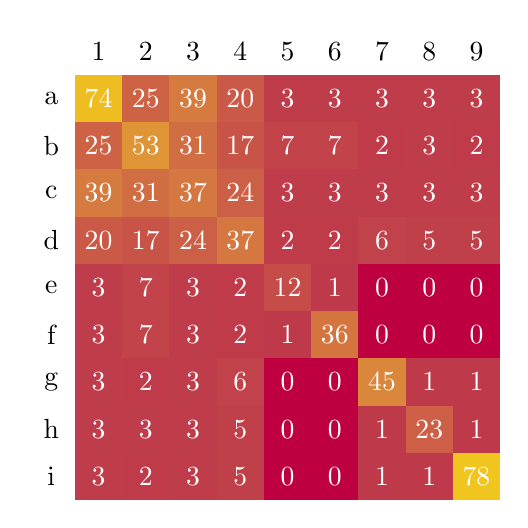
\begin{tikzpicture}[scale=0.6]
  \foreach \y [count=\n] in {
      {74,25,39,20,3,3,3,3,3},
      {25,53,31,17,7,7,2,3,2},
      {39,31,37,24,3,3,3,3,3},
      {20,17,24,37,2,2,6,5,5},
      {3,7,3,2,12,1,0,0,0},
      {3,7,3,2,1,36,0,0,0},
      {3,2,3,6,0,0,45,1,1},
      {3,3,3,5,0,0,1,23,1},
      {3,2,3,5,0,0,1,1,78},
    } {
      % column labels
      \ifnum\n<10
        \node[minimum size=6mm] at (\n, 0) {\n};
      \fi
      % heatmap tiles
      \foreach \x [count=\m] in \y {
        \node[fill=yellow!\x!purple, minimum size=6mm, text=white] at (\m,-\n) {\x};
      }
    }

  % row labels
  \foreach \a [count=\i] in {a,b,c,d,e,f,g,h,i} {
    \node[minimum size=6mm] at (0,-\i) {\a};
  }
\end{tikzpicture}
\end{document}
